\documentclass[../main.tex]{subfiles}
\graphicspath{{\subfix{../images/}}}
\begin{document}

\section{Our Friend, the Stick Figure}

\begin{tabular}{p{2cm}p{9.5cm}}
      \raisebox{-1\totalheight}{  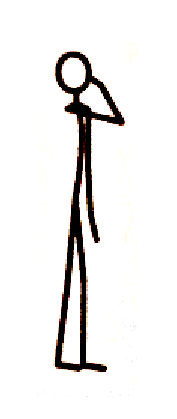
\includegraphics[width=2cm]{water} } \label{sf:water} &

The stick figure accompanies us on the journey into the world of stress. He has been a passionate, willing and good model.
He appeared first in the exercises PACE, the equilibrium exercises and the tibetan rites in the original notes of my mentor Kilian Schmidt.
One of his students illustrated these exercises for him and that's where the stick figure was born and came into my life.

He eagerly agreed to continue with me as his artist and if I to be trust his feedback, he had as much fun working with me as me with him.
  It has been a lot of fun have him show you, dear reader, how the exercises look like and much more.
  \end{tabular}

He shows up in the following places:
\begin{description}
\item[Demonstrating stress] (Chapter~\ref{sf:edge} p.~\pageref{sf:edge} ---
  \textbf{No stick figures have been hurt in the production of this book}),
  then Eustress and Distress (p.~\pageref{sf:eustress}) and 
  coping (p.~\pageref{sf:coping}).
  Later on he demonstrates the sun salutation (p.~\pageref{sf:yoga} and the sitting meditation (Chapter~\ref{sf:sm_chair}, p.~\pageref{sf:sm_chair})
\item[In the unit Learning and Learning training] he's back to demonstrate the exercises: the equilibrium exercises (p.~\pageref{sf:equil}),
  the headstand and the preliminary exercises (p.~\pageref{sf:headstand}),
  two of the tibetan rites (p.~\pageref{sf:tibetan})
  and the PACE exercise series (p.~\pageref{sf:PACE}).
\end{description}



\end{document}